% ============================================================================
%  Comparative analysis: our USRP CSI pilot vs published WiFi sensing datasets
%  Build:  pdflatex comparative_analysis.tex   (run twice)
%  Figures: ./figures/*.pdf  (generated by make_figures.py)
% ============================================================================
\PassOptionsToPackage{table}{xcolor}   % enables \rowcolor / \cellcolor
\documentclass[aspectratio=169,10pt]{beamer}

\usetheme{default}
\usecolortheme{seahorse}
\setbeamertemplate{navigation symbols}{}
\setbeamertemplate{footline}[frame number]
\setbeamercolor{frametitle}{fg=black,bg=gray!18}
\setbeamerfont{frametitle}{size=\large,series=\bfseries}
\setbeamercolor{block title}{bg=gray!22,fg=black}
\setbeamercolor{block body}{bg=gray!8}

\usepackage[utf8]{inputenc}
\usepackage{booktabs}
\usepackage{graphicx}
\usepackage{xcolor}
\usepackage{amssymb}
\usepackage{array}

\definecolor{good}{HTML}{1E8449}
\definecolor{warn}{HTML}{B9770E}
\definecolor{bad}{HTML}{922B21}
\definecolor{ours}{HTML}{C0392B}

\newcommand{\yes}{\textcolor{good}{$\checkmark$}}
\newcommand{\may}{\textcolor{warn}{$\sim$}}
\newcommand{\no}{\textcolor{bad}{$\times$}}
\newcommand{\gd}[1]{\textcolor{good}{#1}}
\newcommand{\wn}[1]{\textcolor{warn}{#1}}
\newcommand{\bd}[1]{\textcolor{bad}{#1}}

\title{\bfseries Did we collect our CSI data correctly?}
\subtitle{A comparative analysis of the USRP N210 pilot dataset\\against published WiFi sensing benchmarks}
\author{CSI Human Activity Recognition project}
\date{Pilot captured 17 July 2026 \quad$\cdot$\quad Analysis 20 July 2026}

\begin{document}

\frame{\titlepage}

% ---------------------------------------------------------------- 1
\begin{frame}{The question, and the short answer}
\begin{block}{\small What we asked}
\small We captured 8 CSI takes on a USRP N210 and got 98--99\% accuracy.
Is the \emph{data} actually sound, or did we get a good number for the wrong reasons?
\end{block}

\vspace{0.2em}
\begin{columns}[T]
\column{0.48\textwidth}
\textbf{\gd{What holds up}}
\begin{itemize}\scriptsize
\item Capture rate is \gd{sufficient} for the physics of this task --- proven, not assumed (slide 9)
\item Motion signal is \gd{strong and real}: $4.2\times$ energy separation
\item Evaluation protocol is \gd{stricter} than ARIL's and UT-HAR's
\item Front-end choices \gd{match} a published USRP dataset (ARIL)
\end{itemize}

\column{0.48\textwidth}
\textbf{\bd{What does not}}
\begin{itemize}\scriptsize
\item Task is \bd{nearly trivial}: \textbf{one scalar gets 99.1\%}. Our 98--99\% proves the pipeline, not the model
\item \bd{13\% of windows silently discarded} by a preprocessing misconfiguration
\item \bd{$4\times$--$800\times$ smaller} than reference datasets
\item 2 subjects, 1 room, 1 day $\Rightarrow$ \bd{no domain diversity}
\end{itemize}
\end{columns}

\vspace{0.2em}
\begin{block}{\small Verdict}
\small\textbf{The collection method is sound and the pilot passes.}
The accuracy is real but \emph{uninformative} --- it validates the chain, not the approach.
The 7-class plan needs the slide-16 fixes.
\end{block}
\end{frame}

% ---------------------------------------------------------------- 2
\begin{frame}{What we collected}
\begin{columns}[T]
\column{0.55\textwidth}
\small
\textbf{Setup.} USRP N210 \emph{passively sniffs} an existing MacBook\,$\rightarrow$\,Android-hotspot
802.11 link. Channel 11 (2.462\,GHz), 20\,MHz, single antenna.
52 OFDM subcarriers, amplitude only.

\vspace{0.5em}
\textbf{Task.} Binary: \texttt{action} (person moving) vs \texttt{noaction}
(person present but still). Presence is held constant on purpose --- the model
must learn \emph{motion}, not \emph{occupancy}.

\vspace{0.5em}
\textbf{Takes.} 2 subjects $\times$ 4 takes $\times$ $\approx$90\,s:
\texttt{walk}, \texttt{mixed} (squat\,$\rightarrow$\,bend\,$\rightarrow$\,drink\,$\rightarrow$\,side-steps,
$\approx$18--20\,s loop), \texttt{stand}, \texttt{sit}.

\column{0.43\textwidth}
\vspace{-0.6em}
\begin{table}\scriptsize
\begin{tabular}{@{}llrr@{}}
\toprule
\textbf{Take} & \textbf{Subject} & \textbf{Hz} & \textbf{s}\\
\midrule
\rowcolor{red!6} walk  & rishiikesh & 77.6 & 91.6\\
\rowcolor{red!6} mixed & rishiikesh & 56.1 & 95.9\\
\rowcolor{red!6} walk  & amrith     & 73.0 & 91.9\\
\rowcolor{red!6} mixed & amrith     & 73.5 & 107.9\\
\rowcolor{blue!6} stand & rishiikesh & 62.9 & 89.8\\
\rowcolor{blue!6} sit   & rishiikesh & 51.5 & 90.9\\
\rowcolor{blue!6} stand & amrith     & 65.6 & 92.1\\
\rowcolor{blue!6} sit   & amrith     & 71.0 & 91.8\\
\midrule
\multicolumn{2}{@{}l}{\textbf{total}} & \textbf{66.4} & \textbf{752}\\
\bottomrule
\end{tabular}
\end{table}
\scriptsize\textcolor{gray}{red = action, blue = noaction. 322 windows of 2\,s survived segmentation.}
\end{columns}

\vspace{0.2em}
\begin{block}{\small Data hygiene check}
\scriptsize
Every file carries \textbf{exactly one truncated final row} (Ctrl+C landed mid-write) ---
361 empty cells out of 3.1\,M, i.e.\ \gd{0.015\%}. No zero rows, no constant or dead
subcarriers. \textbf{Cosmetic, not a data-quality problem}; drop the last row.
\end{block}
\end{frame}

% ---------------------------------------------------------------- 3
\begin{frame}{Which datasets we compare against, and why}
\footnotesize
Three published datasets that bracket our setup from different directions.
All quoted figures are the authors' published specifications.

\vspace{0.4em}
\begin{block}{\small ARIL (2019) --- the hardware twin}
\footnotesize Ettus \textbf{USRP N210}, \textbf{52 subcarriers}, \textbf{single TX/RX link},
\textbf{amplitude only}, segments linearly interpolated to fixed length.
\emph{Almost every low-level choice matches ours.} Difference: they \emph{control} both ends
(two USRPs + OctoClock GPS sync); we sniff a live link passively.
6 hand gestures, 16 locations, \textbf{1 volunteer}, 1394 samples.
\end{block}

\begin{block}{\small UT-HAR / Yousefi et al.\ (2017) --- the task twin}
\footnotesize Intel 5300 NIC, $30\times3=90$ streams, \textbf{1\,kHz}. Seven whole-body activities
(walk, run, fall, sit down, stand up, lie down, pick up) --- the closest published task to
our eventual 7-class plan. 6 subjects, $\approx$4{,}477 samples.
\end{block}

\begin{block}{\small Widar 3.0 (2019) --- the gold standard}
\footnotesize Intel 5300, 1 TX + 6 RX $\times$ 3 antennas $=$ \textbf{18 links} $\times$ 30 subcarriers,
\textbf{1\,kHz}. 22 gestures, \textbf{16 subjects, 75 domains}, \textbf{258k instances}.
Uses \emph{phase} across antennas for Doppler (DFS) and velocity profiles (BVP) ---
which our single-antenna setup structurally cannot reproduce.
\end{block}
\end{frame}

% ---------------------------------------------------------------- 4
\begin{frame}{Head-to-head specification table}
\centering
\begin{table}\scriptsize
\begin{tabular}{@{}l|c|ccc@{}}
\toprule
 & \cellcolor{red!12}\textbf{Ours (pilot)} & \textbf{ARIL} & \textbf{UT-HAR} & \textbf{Widar 3.0}\\
\midrule
Radio & \cellcolor{red!6}USRP N210 & USRP N210 $\times2$ & Intel 5300 & Intel 5300\\
Acquisition & \cellcolor{red!6}\textbf{passive sniff} & controlled TX+RX & controlled & controlled\\
Sync / clock & \cellcolor{red!6}none & OctoClock GPS & NIC & NIC\\
\midrule
Subcarriers & \cellcolor{red!6}52 & 52 & 30 & 30\\
Links $\times$ antennas & \cellcolor{red!6}\bd{1 (SISO)} & 1 (SISO) & 3 & \gd{18}\\
Total CSI streams & \cellcolor{red!6}\bd{52} & 52 & 90 & \gd{540}\\
\midrule
Packet rate & \cellcolor{red!6}\wn{51--78\,Hz} & not reported & \gd{1000\,Hz} & \gd{1000\,Hz}\\
Nyquist (worst) & \cellcolor{red!6}\wn{25.7\,Hz} & --- & 500\,Hz & 500\,Hz\\
\midrule
Uses phase & \cellcolor{red!6}\no\ (unsynced) & \no\ (discarded) & \no & \yes\ DFS/BVP\\
Classes & \cellcolor{red!6}\bd{2} & 6 & 7 & \gd{22}\\
Subjects & \cellcolor{red!6}\bd{2} & \bd{1} & 6 & \gd{16}\\
Rooms / domains & \cellcolor{red!6}\bd{1} & 16 positions & 1 & \gd{75}\\
Days & \cellcolor{red!6}\bd{1} & n/r & n/r & multiple\\
Labelled samples & \cellcolor{red!6}\bd{322} & 1{,}394 & 4{,}477 & \gd{258{,}000}\\
\midrule
Test split & \cellcolor{red!6}\gd{\textbf{leave-one-subject-out}} & \bd{every 5th sample} & \bd{random} & \gd{cross-domain}\\
\bottomrule
\end{tabular}
\end{table}

\vspace{0.2em}
\scriptsize
\textbf{Read this honestly:} we lose badly on \emph{scale} and \emph{diversity}, we match ARIL on
\emph{front-end design}, and we are the \emph{only one of the four} whose headline number comes from a
subject-independent split.
\end{frame}

% ---------------------------------------------------------------- 5
\begin{frame}{Capture rate --- the headline weakness}
\centering
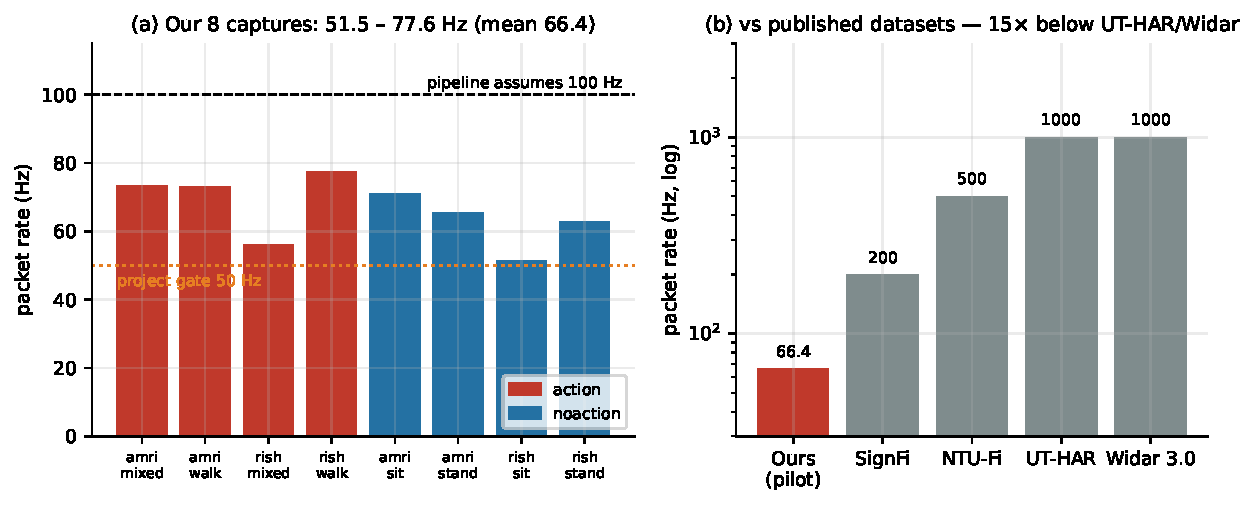
\includegraphics[width=0.86\textwidth]{figures/fig1_rate.pdf}

\vspace{0.2em}
\begin{columns}[T]
\column{0.5\textwidth}
\scriptsize
\textbf{Measured:} 51.5--77.6\,Hz, mean \textbf{66.4\,Hz}.
All 8 takes clear the project's own 50\,Hz gate, but every take is
\emph{below} the 100\,Hz the preprocessing pipeline assumes.

\column{0.5\textwidth}
\scriptsize
\textbf{Cause:} we sniff a real link opportunistically. Rate is set by how many
frames the MacBook emits \emph{and} that \texttt{gr-ieee802-11} can decode
(legacy OFDM only; 802.11n HT frames are dropped).
Widar/UT-HAR simply command a 1\,kHz injector.
\end{columns}

\vspace{0.2em}
\begin{block}{\small But is 66\,Hz actually too slow? --- see slide 9 before concluding}
\scriptsize It is $15\times$ below UT-HAR. That sounds fatal. Measured against the
\emph{physics of what we are sensing}, it turns out not to be --- for \emph{this} task.
\end{block}
\end{frame}

% ---------------------------------------------------------------- 6
\begin{frame}{Rate stability --- where the dropped windows came from}
\centering
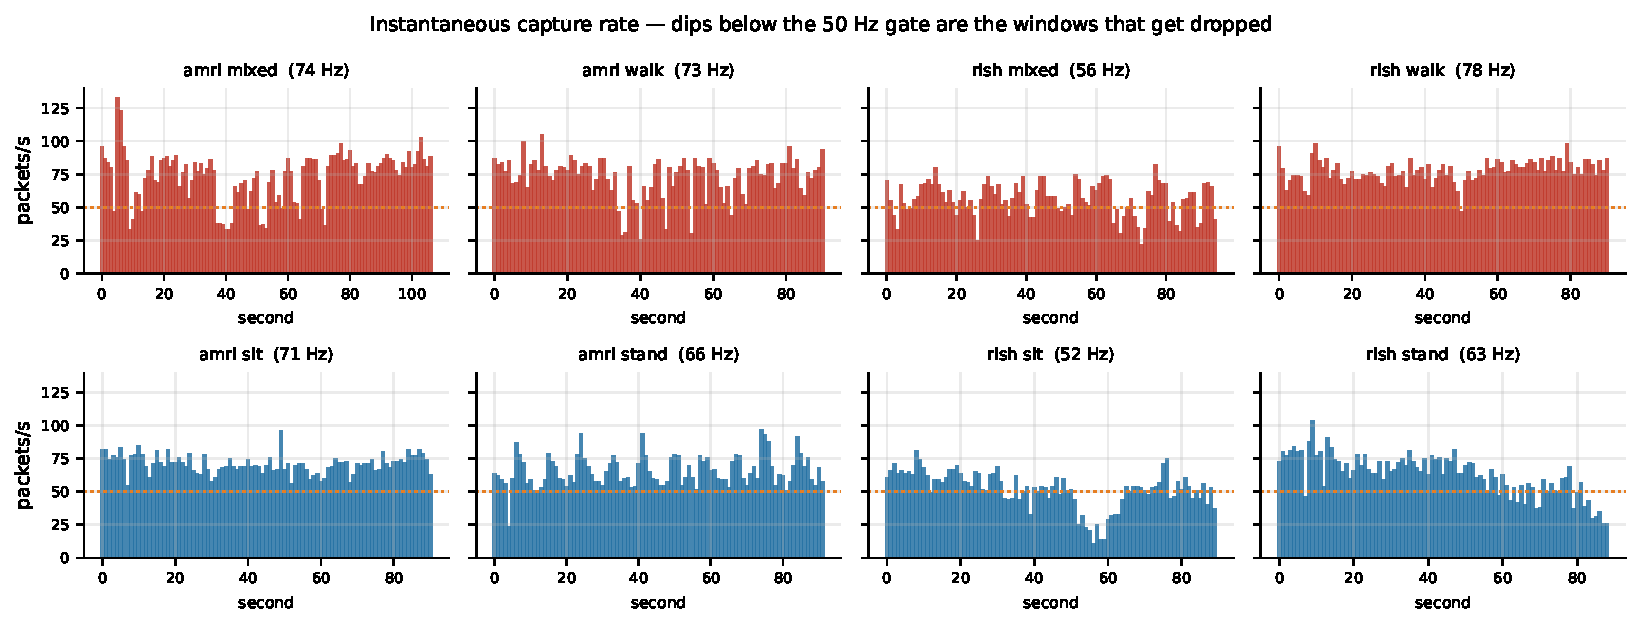
\includegraphics[width=0.95\textwidth]{figures/fig2_rate_stability.pdf}

\vspace{0.2em}
\footnotesize
Rate is \emph{not} steady. Per-second minima fall to \textbf{11--55 packets/s}
(\texttt{rishiikesh sit} bottoms out at 11). Every dip below the segmenter's
fill threshold silently deletes a 2\,s window.
\textbf{This is a capture-side artefact of passive sniffing}, not a bug ---
but it must be budgeted for, not ignored.
\end{frame}

% ---------------------------------------------------------------- 7
\begin{frame}{Timing jitter and the 13\% we threw away}
\centering
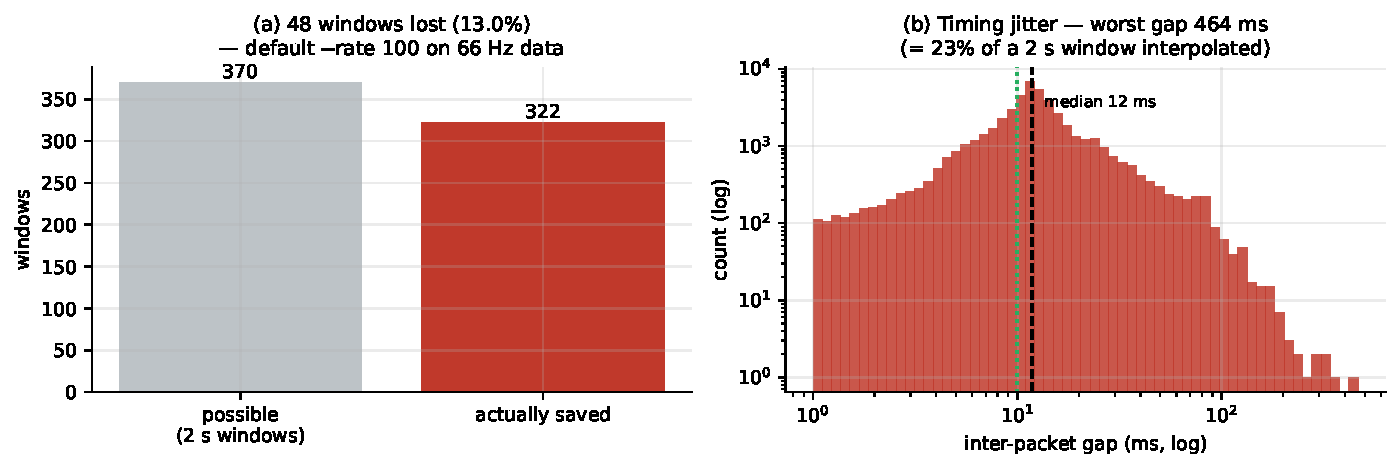
\includegraphics[width=0.92\textwidth]{figures/fig10_yield.pdf}

\vspace{0.3em}
\begin{columns}[T]
\column{0.5\textwidth}
\footnotesize
\textbf{\bd{A real, fixable mistake.}}
\texttt{segment\_all\_pilot.py} ran \texttt{segment\_windows.py} at its
\emph{default} \texttt{-{}-rate 100}. On 66\,Hz data each 2\,s window then needs
$\ge$100 packets to survive; many did not.

\vspace{0.3em}
752\,s of capture $\Rightarrow$ 370 possible windows,
\textbf{322 saved, 48 lost (13.0\%)}.

\column{0.5\textwidth}
\footnotesize
\textbf{Fix:} pass \texttt{-{}-rate 50}. Threshold drops to 50 packets/2\,s,
which every take clears. \gd{Recovers $\approx$48 windows ($+15\%$ data) for free},
with no recapture.

\vspace{0.3em}
\textbf{Jitter:} median gap 11--14\,ms, but the 99th percentile reaches 99\,ms and the
worst gap is \bd{464\,ms} --- 23\% of a 2\,s window filled by interpolation across a hole.
\end{columns}
\end{frame}

% ---------------------------------------------------------------- 8
\begin{frame}{The signal itself is real}
\centering
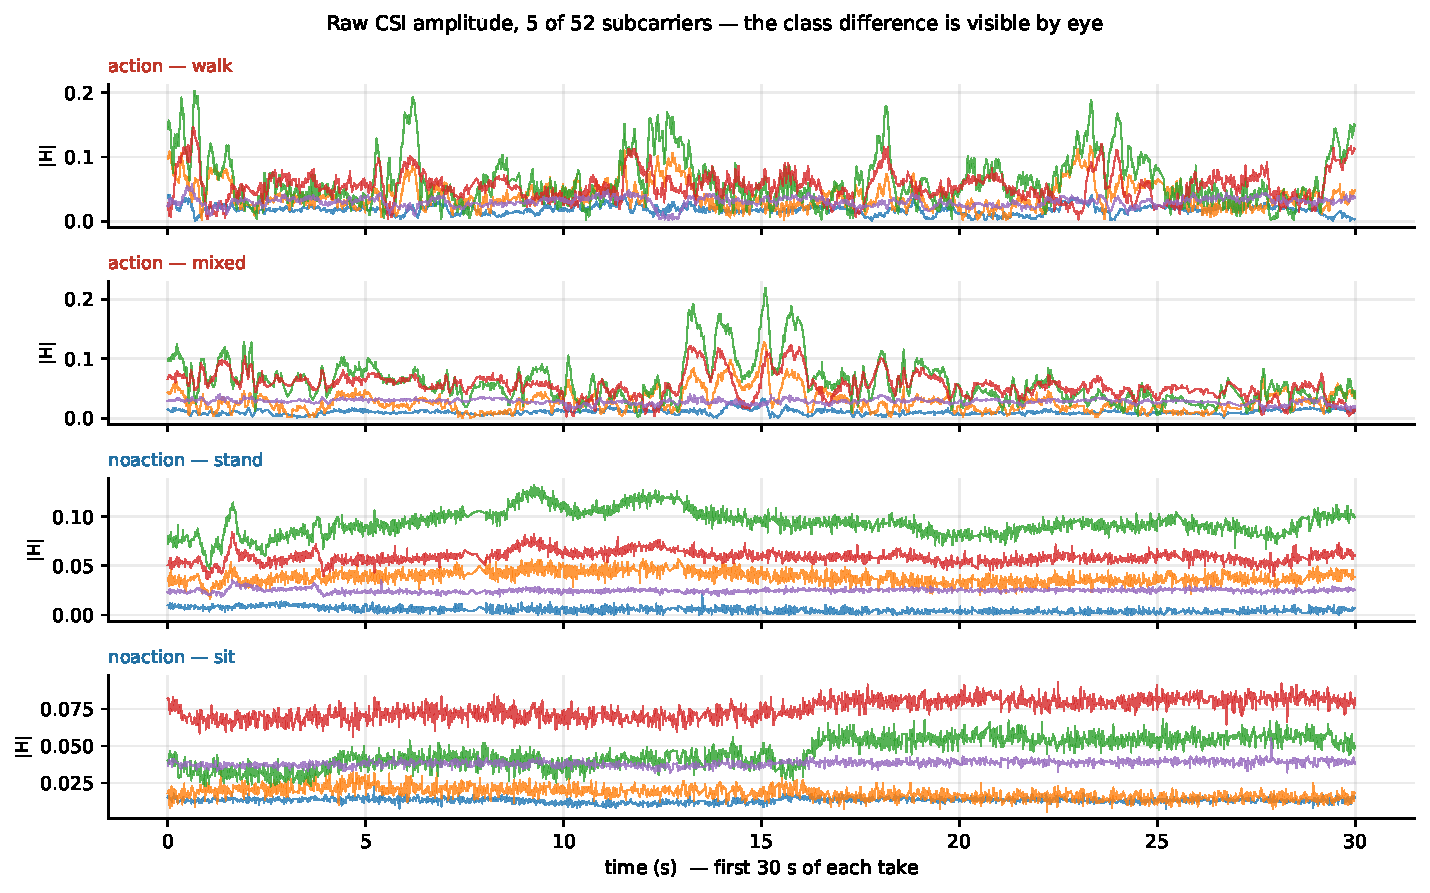
\includegraphics[height=0.68\textheight]{figures/fig3_traces.pdf}

\vspace{0.1em}
\scriptsize
The project's own ``wiggle test'' criterion --- \emph{if you cannot see it by eye, the network cannot either} ---
is comfortably met. \texttt{walk} and \texttt{mixed} show large multi-scale fluctuation;
\texttt{stand} and \texttt{sit} are visibly flat (residual ripple is breathing plus noise).
\end{frame}

% ---------------------------------------------------------------- 9
\begin{frame}{Is 66\,Hz enough? Measuring, not guessing}
\centering
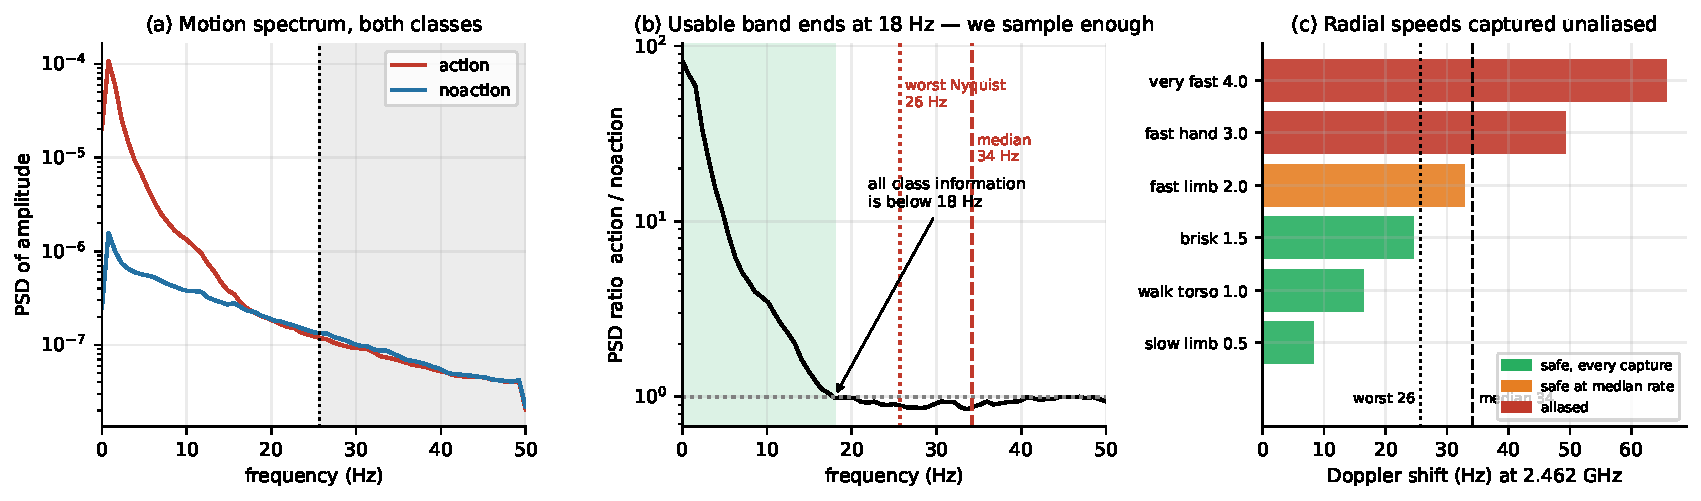
\includegraphics[width=0.93\textwidth]{figures/fig5_doppler.pdf}

\vspace{0.15em}
\begin{block}{\small The key result of this analysis}
\scriptsize
Panel (b) divides the \texttt{action} spectrum by the \texttt{noaction} spectrum.
Above \textbf{18\,Hz the ratio is 1.0} --- the classes are \emph{indistinguishable}; that band is
pure noise floor. \textbf{All class-discriminative information lives below 18\,Hz.}
Our worst-case Nyquist is \textbf{25.7\,Hz}, median \textbf{34\,Hz}
$\Rightarrow$ \gd{\textbf{we sample the informative band with $1.4$--$1.9\times$ headroom.}}
The 15$\times$ rate deficit versus UT-HAR costs \emph{nothing measurable on this task}.
\end{block}

\vspace{0.1em}
\scriptsize
\wn{\textbf{Caveat for the 7-class plan:}} this holds because \texttt{walk} and
\texttt{mixed} are gross whole-body motions (Doppler $\le$25\,Hz, panel c).
A fast hand (3\,m/s $\rightarrow$ 49\,Hz) or a \texttt{nod} lands \emph{outside} this band and
aliases. \textbf{We have not yet proven those classes are capturable at 66\,Hz.}
\end{frame}

% ---------------------------------------------------------------- 10
\begin{frame}{How separable are the classes, really?}
\centering
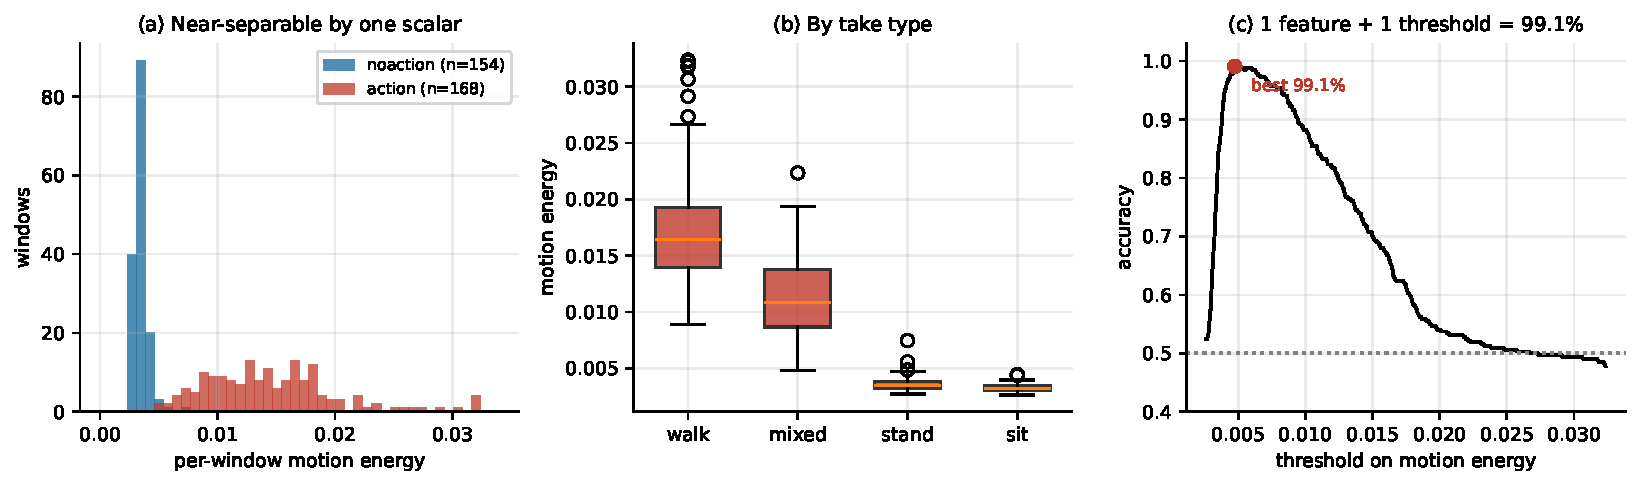
\includegraphics[width=0.97\textwidth]{figures/fig4_energy.pdf}

\vspace{0.3em}
\begin{block}{\small The uncomfortable finding --- state this to anyone quoting our accuracy}
\footnotesize
Take one scalar per window: mean over subcarriers of the temporal standard deviation
(``motion energy''). \texttt{action} averages $4.20\times$ \texttt{noaction}
(0.0145 vs 0.0035), Fisher ratio 3.85.

\textbf{A single threshold on that one number classifies 99.1\% of windows correctly.}
\end{block}

\vspace{0.2em}
\footnotesize
Our CNN--GRU--Attention model scores 98.4--99.3\%. \bd{\textbf{It does not beat the
one-line baseline.}} That is not a failure of the model --- it means \emph{this binary task
cannot discriminate between a good model and a trivial one}.
Per-take energies (panel b) show why: \texttt{walk} 0.0174 and \texttt{mixed} 0.0114 sit far above
\texttt{stand} 0.0036 and \texttt{sit} 0.0033.
\end{frame}

% ---------------------------------------------------------------- 11
\begin{frame}{52 subcarriers, but how many independent views?}
\centering
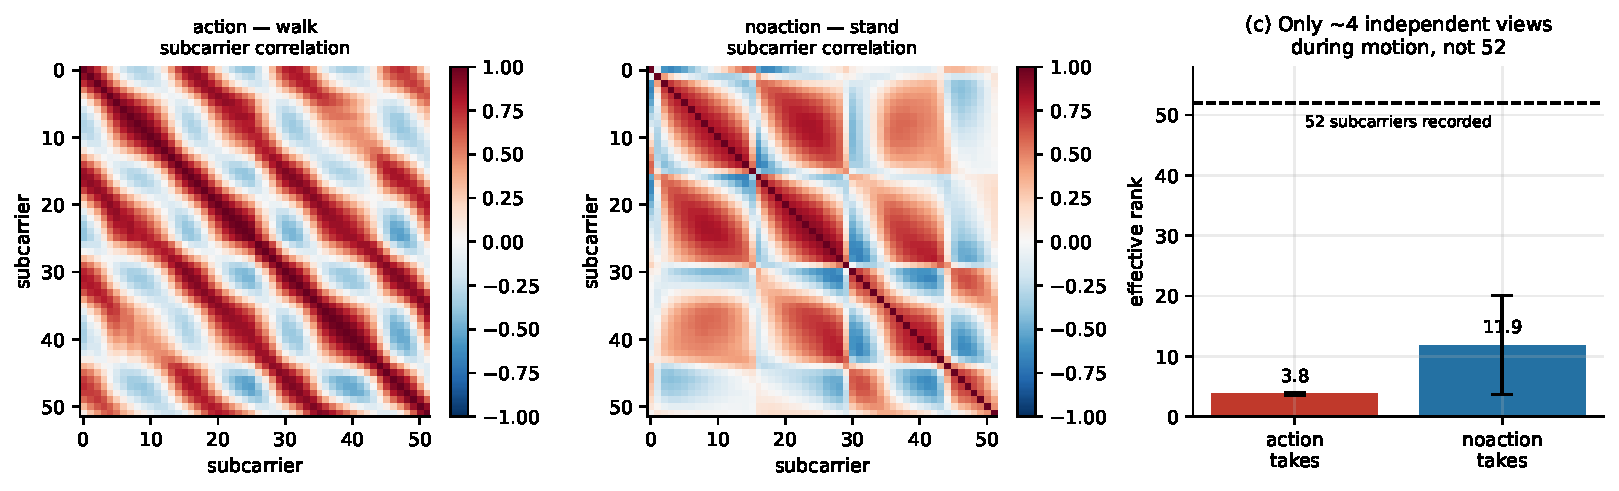
\includegraphics[width=0.95\textwidth]{figures/fig6_redundancy.pdf}

\vspace{0.3em}
\begin{columns}[T]
\column{0.52\textwidth}
\footnotesize
Neighbouring subcarriers are strongly correlated (mean $|r|$ = 0.38--0.45 during motion).
Effective rank of the 52-dimensional covariance:
\textbf{3.5--4.2 during \texttt{action}}, 5.6--25.7 during \texttt{noaction}.

\vspace{0.3em}
A moving body imposes \emph{one} dominant channel perturbation that all subcarriers see
together --- so 52 measurements carry roughly \textbf{4 independent dimensions}.

\column{0.46\textwidth}
\footnotesize
\textbf{Why this matters.} The ImgFi recipe multiplies the dataset $\times52$ by making one
recurrence image per subcarrier and calls it free data.
\bd{It is not free: those 52 images are $\approx$4 distinct views plus 48 near-duplicates.}

\vspace{0.3em}
The effective dataset is closer to \textbf{322 windows $\times$ 4}, not $\times$52.
This is a strong argument for the team's move to the
\gd{whole-matrix CNN--GRU model}, which consumes all 52 jointly instead of voting over them.
\end{columns}
\end{frame}

% ---------------------------------------------------------------- 12
\begin{frame}{What the model actually sees, and what it scored}
\centering
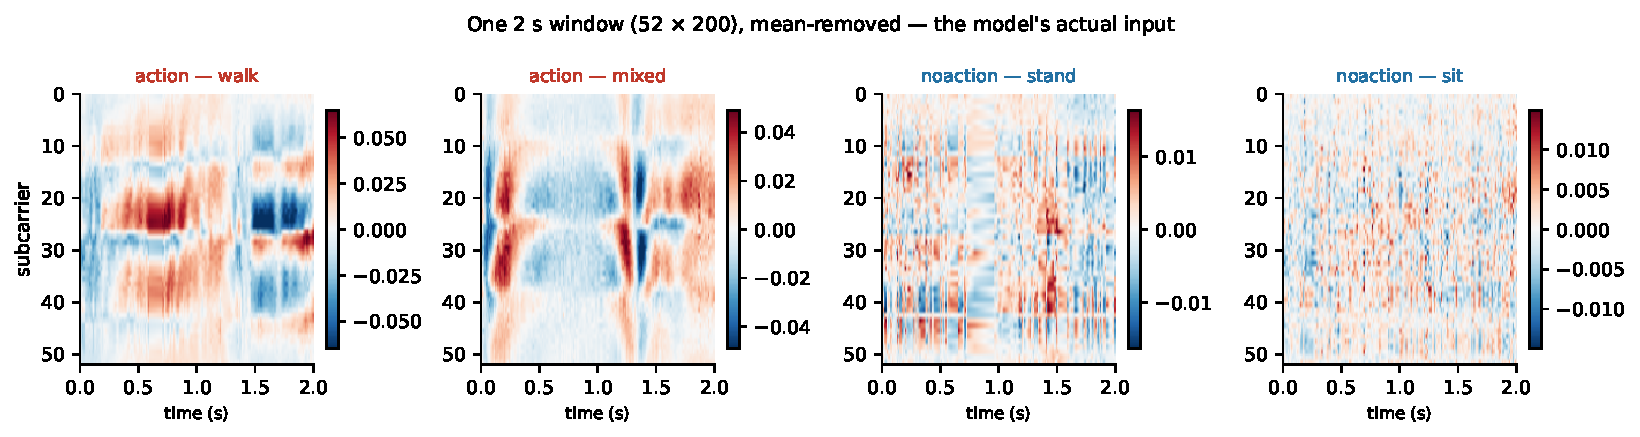
\includegraphics[width=0.92\textwidth]{figures/fig7_windows.pdf}

\vspace{0.4em}
\begin{columns}[c]
\column{0.42\textwidth}
\centering
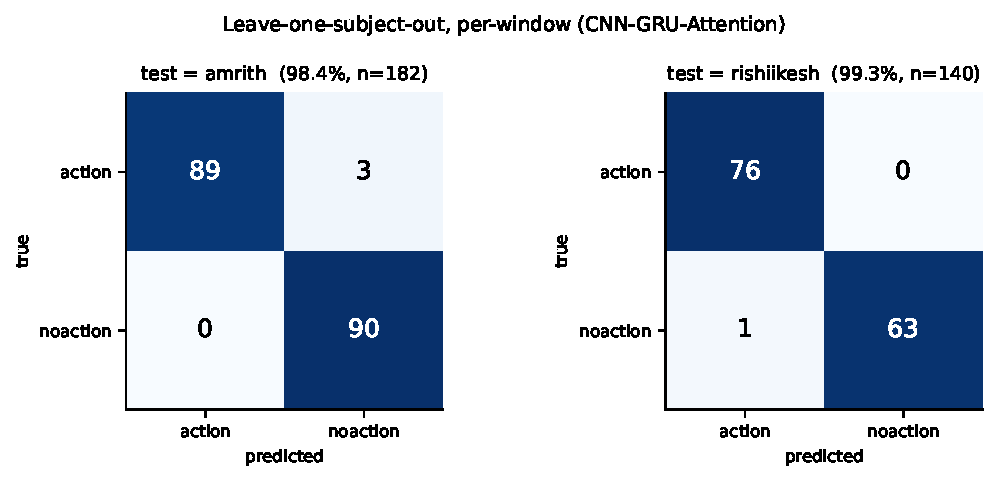
\includegraphics[width=\textwidth]{figures/fig9_confusion.pdf}

\column{0.56\textwidth}
\footnotesize
\textbf{Leave-one-subject-out, per window:}
\begin{itemize}
\item test = amrith: \textbf{98.4\%} (179/182)
\item test = rishiikesh: \textbf{99.3\%} (139/140)
\item \textbf{Headline (worse of the two): 98.4\%}
\end{itemize}

\vspace{0.3em}
Against the pilot's own pass bar ($\ge$95\% $\Rightarrow$ green light) this
\gd{passes clearly}. Only 4 errors in 322 windows, and errors are not
concentrated in one class.

\vspace{0.3em}
\wn{Read together with slide 10:} a 1-feature baseline gets 99.1\% on the same data.
\end{columns}
\end{frame}

% ---------------------------------------------------------------- 13
\begin{frame}{Scale and diversity --- where we are genuinely behind}
\centering
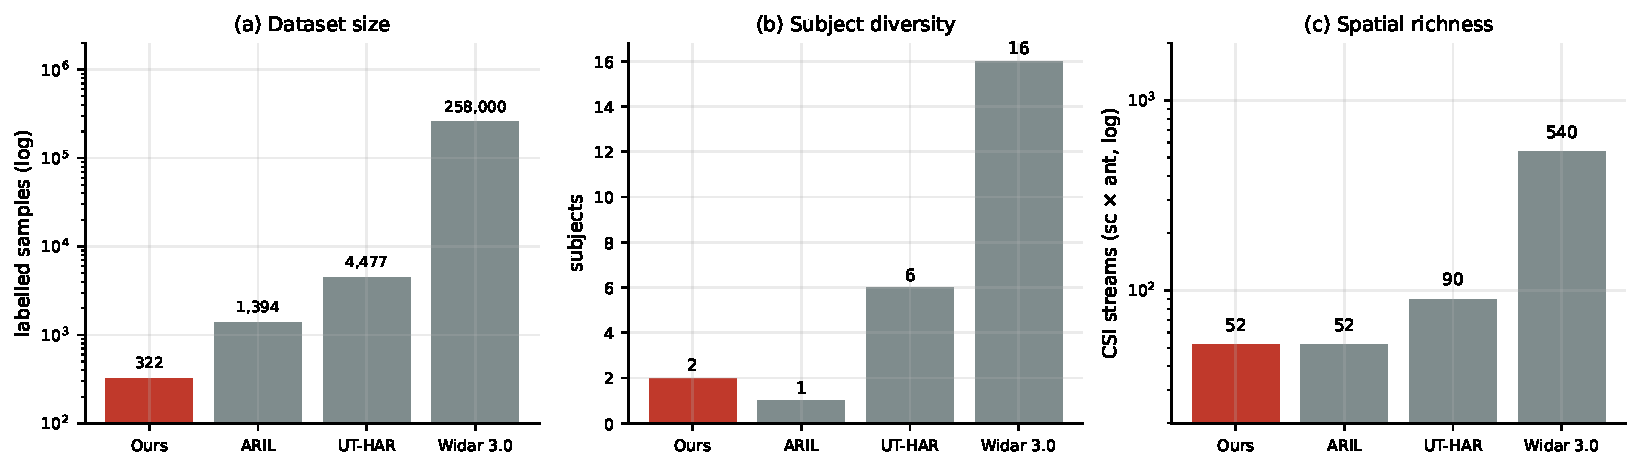
\includegraphics[width=0.95\textwidth]{figures/fig8_scale.pdf}

\vspace{0.2em}
\scriptsize
\begin{itemize}\itemsep2pt
\item \textbf{Volume.} 322 samples vs 1{,}394 (ARIL), 4{,}477 (UT-HAR), 258{,}000 (Widar 3.0)
--- $4\times$ to $800\times$ smaller.
\item \textbf{Subjects.} 2 --- exactly one leave-one-subject-out fold each direction,
with no third subject to confirm the result generalises.
\item \textbf{Domains.} One room, one geometry, one orientation, one evening.
Widar's entire contribution is the \emph{75 domains} that expose how badly WiFi sensing
overfits to environment. \bd{We cannot detect that failure mode at all.}
\item \textbf{Streams.} 52 vs Widar's 540. Single-antenna SISO also means
\bd{no antenna-pair phase difference} $\Rightarrow$ DFS/BVP features are unavailable
in principle, not merely unimplemented.
\end{itemize}
\end{frame}

% ---------------------------------------------------------------- 14
\begin{frame}{Where our methodology is stronger than the references}
\footnotesize
Being honest cuts both ways. On evaluation protocol we are the strictest of the four.

\vspace{0.3em}
\begin{table}\scriptsize
\begin{tabular}{@{}lll@{}}
\toprule
\textbf{Dataset} & \textbf{Reported split} & \textbf{Leakage risk}\\
\midrule
\rowcolor{green!8}\textbf{Ours} & leave-one-subject-out & \gd{none --- subject never seen in training}\\
ARIL & every 5th sample to test & \bd{high} --- same volunteer, same session, adjacent reps\\
UT-HAR & random train/test & \bd{high} --- overlapping sliding windows can straddle the split\\
Widar 3.0 & cross-domain & \gd{low} --- explicit unseen room/orientation/user protocols\\
\bottomrule
\end{tabular}
\end{table}

\vspace{0.3em}
\begin{block}{\small Two design decisions that were correct}
\scriptsize
\textbf{1. Amplitude only.} Our USRP is not synchronised to the MacBook, so raw phase is
scrambled by CFO/SFO/timing offset. We discard it. \emph{ARIL discards phase too --- even
though they had OctoClock GPS sync and controlled both ends.} Independent confirmation
that this was the right call.

\vspace{0.2em}
\textbf{2. Person present in both classes.} \texttt{noaction} is a still \emph{person},
not an empty room. This forces the model to learn motion rather than occupancy --- a
harder and far more useful problem than the trivial version.
\end{block}
\end{frame}

% ---------------------------------------------------------------- 15
\begin{frame}{Honest scorecard}
\centering
\begin{table}\scriptsize
\begin{tabular}{@{}p{0.30\textwidth} c p{0.53\textwidth}@{}}
\toprule
\textbf{Aspect} & & \textbf{Assessment}\\
\midrule
Hardware / front-end & \yes & Matches ARIL, a peer-reviewed USRP dataset, spec for spec\\
Amplitude-only choice & \yes & Correct and independently corroborated\\
Sampling adequacy & \yes & Measured $1.4$--$1.9\times$ headroom over the 18\,Hz informative band\\
Signal strength & \yes & $4.2\times$ energy separation; visible by eye\\
Class design & \yes & Motion-vs-stillness with presence held constant\\
Evaluation protocol & \yes & Strictest of the four datasets compared\\
Data hygiene & \yes & 0.015\% truncated cells; otherwise clean\\
\midrule
Rate stability & \may & Dips to 11--55\,pkt/s; gaps to 464\,ms\\
Window yield & \may & 13\% lost to a preprocessing default --- recoverable without recapture\\
Subcarrier redundancy & \may & $\approx$4 effective dimensions, not 52\\
\midrule
Task difficulty & \no & 99.1\% from one scalar $\Rightarrow$ accuracy proves nothing about the model\\
Dataset size & \no & $4$--$800\times$ smaller than references\\
Subject diversity & \no & 2 subjects; ARIL has 1, but Widar has 16\\
Domain diversity & \no & 1 room, 1 day, 1 geometry --- overfitting is undetectable\\
Spatial diversity & \no & SISO; no DFS/BVP possible even in principle\\
\bottomrule
\end{tabular}
\end{table}
\end{frame}

% ---------------------------------------------------------------- 16
\begin{frame}{What to change before the 7-class collection}
\footnotesize
\begin{block}{\small Must fix --- costs nothing}
\scriptsize
\begin{enumerate}\itemsep1pt
\item \textbf{Segment with \texttt{-{}-rate 50}}, not the default 100. Recovers $\approx$13\% of windows immediately.
\item \textbf{Always report a trivial baseline} (motion energy + threshold, or a small
random forest) beside the deep model. If the gap is not large, the task is too easy to
justify the architecture.
\item \textbf{Drop the truncated last row} of every capture in the loader.
\item \textbf{Fix \texttt{segment\_all\_pilot.py}'s glob:} it matches \texttt{*.csv}, so the
\texttt{*\_confusion.csv} files now sitting in \texttt{data/pilot/} would be parsed as captures and
create a bogus \texttt{windows/model/} class. Restrict it to \texttt{P01\_*.csv}.
\end{enumerate}
\end{block}

\begin{block}{\small Must fix --- costs collection time}
\scriptsize
\begin{enumerate}\itemsep1pt\setcounter{enumi}{4}
\item \textbf{Pre-flight each new class before bulk collection.} Record 30\,s of \texttt{nod} and
\texttt{drink} and run the slide-9 spectral-ratio test. If a class has no
\texttt{action}/\texttt{noaction} ratio above 1 inside 0--25\,Hz, \emph{it is not
capturable at our rate} --- find that out in 10 minutes, not after a full session.
\item \textbf{Raise the packet rate if that test fails.} Force legacy-OFDM traffic,
shorter ping interval, or inject with a second USRP as ARIL did.
\item \textbf{$\ge$5 subjects, $\ge$2 days, $\ge$2 room geometries.} Without a second day
and a second geometry we cannot measure the failure mode Widar exists to expose.
\item \textbf{Use \texttt{-{}-step 1.0}} for 50\% window overlap --- roughly doubles sample count
at zero capture cost (train-side only; keep test windows non-overlapping).
\end{enumerate}
\end{block}
\end{frame}

% ---------------------------------------------------------------- 17
\begin{frame}{Conclusion}
\begin{block}{\small Did we collect the data correctly?}
\footnotesize
\textbf{Yes.} The front-end design, the amplitude-only decision, the class definitions and the
evaluation protocol are all sound, and several match or exceed published practice.
The one concrete error --- segmenting 66\,Hz data with a 100\,Hz assumption --- is fixable
without recapturing anything.
\end{block}

\vspace{0.2em}
\begin{block}{\small Does the 98.4\% mean what it looks like?}
\footnotesize
\textbf{No.} It is an honest, leakage-free number, but a single hand-crafted scalar reaches
99.1\% on the same windows. The pilot proves the \emph{chain works end to end}.
It does \emph{not} show that our model, our features, or our sampling rate will
survive 7 classes.
\end{block}

\vspace{0.2em}
\begin{block}{\small What the pilot was for}
\footnotesize
Exactly this. It was designed as a throwaway sanity check, and it did its job:
capture, segmentation, training and honest evaluation all work.
\textbf{Green light for the 7-class collection}, conditional on the slide-16 fixes ---
above all the 10-minute spectral pre-flight on \texttt{nod} and \texttt{drink},
which is where this setup is most likely to fail.
\end{block}
\end{frame}

% ---------------------------------------------------------------- 18
\begin{frame}{References and reproducibility}
\footnotesize
\textbf{Reference datasets} (all figures quoted are published specifications, not re-measured):
\begin{enumerate}
\item F.\ Wang, J.\ Feng, Y.\ Zhao, X.\ Zhang, S.\ Zhang, J.\ Han.
\textit{Joint Activity Recognition and Indoor Localization with WiFi Fingerprints} (ARIL).
IEEE Access, 2019. arXiv:1904.04964.
\item S.\ Yousefi et al.\ \textit{A Survey on Behavior Recognition Using WiFi Channel State
Information} (UT-HAR). IEEE Communications Magazine, 2017.
\item Y.\ Zheng et al.\ \textit{Zero-Effort Cross-Domain Gesture Recognition with Wi-Fi}
(Widar 3.0). ACM MobiSys, 2019.
\item J.\ Yang et al.\ \textit{SenseFi: A library and benchmark on deep-learning-empowered
WiFi human sensing}. Patterns, 2023. (Used for cross-dataset rate/scale figures.)
\end{enumerate}

\vspace{0.5em}
\textbf{Our numbers} --- every pilot figure in this deck is measured, not quoted:
\begin{itemize}
\item \texttt{analysis/analyze\_pilot.py} $\rightarrow$ \texttt{analysis/pilot\_stats.json}
(rates, jitter, correlation, effective rank, separability, window yield)
\item \texttt{analysis/make\_figures.py} $\rightarrow$ \texttt{analysis/figures/*.pdf}
\item Source data: 8 CSVs and 322 windows under \texttt{data/pilot/}
\item Model results read directly from \texttt{hybrid\_model\_test-*\_confusion.csv}
\end{itemize}

\vspace{0.5em}
\textcolor{gray}{Limitation of this analysis: reference datasets are compared on published
specifications. We did not download and re-analyse their raw CSI, so their signal-level
statistics (jitter, effective rank, spectral ratio) are not measured here.}
\end{frame}

\end{document}
